% *********************************************************************
% © 2010–2022 Jeremy Sylvestre
%
% Permission is granted to copy, distribute and/or modify this document
% under the terms of the GNU Free Documentation License, Version 1.3 or
% any later version published by the Free Software Foundation; with no
% Invariant Sections, no Front-Cover Texts, and no Back-Cover Texts. A
% copy of the license is included in the appendix entitled “GNU Free
% Documentation License” that appears in the output document of this
% PreTeXt source code. All trademarks™ are the registered® marks of
% their respective owners.
%
% *********************************************************************

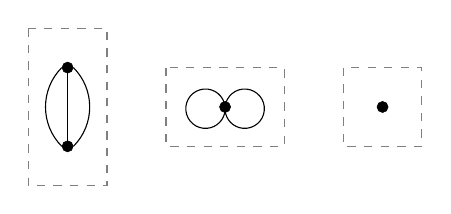
\begin{tikzpicture}[
	vertex/.style={ circle, draw, very thin, fill, inner sep=0pt, minimum size=4pt },
	vertexg/.style={ black!40!white, circle, draw, very thin, fill, inner sep=0pt, minimum size=4pt },
	vertexo/.style={ circle, draw, very thin, inner sep=0pt, minimum size=4pt }
]

\node[vertex] at (0,1) (g2v1) {};
\node[vertex] at (0,0) (g2v2) {};
\draw (g2v2) to (g2v1);
\node[vertex] at (2,0.5) (g2v3) {};
\node[vertex] at (4,0.5) (g2v4) {};
\draw (g2v1.west) to [out=225,in=135] (g2v2.west);
\draw (g2v1.east) to [out=315,in=45] (g2v2.east);
\draw (g2v3) arc (175:-175:0.25cm) to (g2v3);
\draw (g2v3) arc (5:355:0.25cm) to (g2v3);
\draw[dashed,gray] (-0.5,1.5) to (-0.5,-0.5) to (0.5,-0.5) to (0.5,1.5) to (-0.5,1.5);
\draw[dashed,gray] (1.25,1) to (1.25,0) to (2.75,0) to (2.75,1) to (1.25,1);
\draw[dashed,gray] (3.5,1) to (3.5,0) to (4.5,0) to (4.5,1) to (3.5,1);

\end{tikzpicture}
